\documentclass[twoside,11pt]{article}

% Any additional packages needed should be included after jmlr2e.
% Note that jmlr2e.sty includes epsfig, amssymb, natbib and graphicx,
% and defines many common macros, such as 'proof' and 'example'.
%
% It also sets the bibliographystyle to plainnat; for more information on
% natbib citation styles, see the natbib documentation, a copy of which
% is archived at http://www.jmlr.org/format/natbib.pdf

\usepackage{jmlr2e}
% Definitions of handy macros can go here
\usepackage{subfig}
\newcommand{\dataset}{{\cal D}}
\newcommand{\fracpartial}[2]{\frac{\partial #1}{\partial  #2}}

% Heading arguments are {volume}{year}{pages}{submitted}{published}{author-full-names}

% \jmlrheading{1}{2000}{1-48}{4/00}{10/00}{Marina Meil\u{a} and Michael I. Jordan}

% Short headings should be running head and authors last names

% \firstpageno{1}

\begin{document}
\title{COMP 424 Final Project Game: \textit{Colosseum Survival!}}
\ShortHeadings{Final project COMP 424, McGill University}{}
\author{Course Instructor: Jackie Cheung and Bogdan Mazoure \\ Project TAs: Koustuv Sinha (\texttt{koustuv.sinha@mail.mcgill.ca}) and Shuhao Zheng (\texttt{shuhao.zheng@mail.mcgill.ca}) \\ Due Date: April 8th, 2022, 11:59PM EST}

% \author{\name Marina Meil\u{a} \email mmp@stat.washington.edu \\
%       \addr Department of Statistics\\
%       University of Washington\\
%       Seattle, WA 98195-4322, USA
%       \AND
%       \name Michael I.\ Jordan \email jordan@cs.berkeley.edu \\
%       \addr Division of Computer Science and Department of Statistics\\
%       University of California\\
%       Berkeley, CA 94720-1776, USA}

% \editor{Leslie Pack Kaelbling}

\maketitle


% \begin{abstract}%   <- trailing '%' for backward compatibility of .sty file
% Sample Abstract
% \end{abstract}

% \begin{keywords}
%   Bayesian Networks, Mixture Models, Chow-Liu Trees
% \end{keywords}

% \section{Background \cite{ColosseumIconRome,Colosseum2022}}
% \begin{figure}[!htbp]
%     \centering
%     
\includegraphics[width=0.6\textwidth]{Colosseum-Rome-Italy.jpg}
%     \caption{Colosseum \cite{Colosseum}}
% \end{figure}
% %
% The Roman Colosseum, also known as the Flavian Amphitheatre, is one of the capital's most remarkable monuments.
% %
% As the main symbol of Rome, it is an imposing construction with almost 2,000 years of history.
% %
% The construction of the Colosseum began in the year 72 under the empire of Vespasian and was finished in the year 80 during the rule of the emperor Titus.
% %
% After completion, the Colosseum became the greatest Roman amphitheatre, measuring 188 meters in length, 156 meters in width and 57 meters in height.

% %
% During the Roman Empire time, the Roman Colosseum allowed more than 50,000 people to enjoy its finest spectacles.
% %
% The exhibitions of exotic animals, executions of prisoners, recreations of battles and gladiator fights kept the Roman people entertained for years.
% %
% Such events were occasionally on a huge scale.
% %
% Trajan is said to have celebrated his victories in Dacia in 107 with contests involving 11,000 animals and 10,000 gladiators over the course of 123 days.
% %
% During lunch intervals, executions \textit{ad bestias} would be staged.
% %
% Those condemned to death would be sent into the arena, naked and unarmed, to face the beasts of death which would literally tear them to pieces.
% %
% Other performances would also take place by acrobats and magicians, typically during the intervals.
% %
% The Colosseum remained active for over 500 years. The last recorded games in history were celebrated in the 6th century. 

\section{Goal}

The main goal of the project for this course is to give you a chance to play around with some of the AI algorithms discussed in class, in the context of a fun, large-scale problem. This year we will be working on a game called \textbf{\textit{Colosseum Survival!}} (\href{https://github.com/Ctree35/Project-COMP424-2022-Winter}{https://github.com/Ctree35/ Project-COMP424-2022-Winter}). Koustuv Sinha and Shuhao Zheng are in charge of the project, and should be contacted directly about any bugs in the provided code. General questions should be posted in Ed. \textbf{This is a group project, with two students per group}.

\section{Game Description and Rules}
\textit{Colosseum Survival!} is a 2-player turn-based strategy game in which two players move in an $M\times M$ chessboard and put barriers around them until they are separated in two closed zones. $M$ can have a value between $6$ and $12$.
Each player will try to maximize the number of blocks in its zone to win the game.

\begin{figure}[!h]
    \centering
    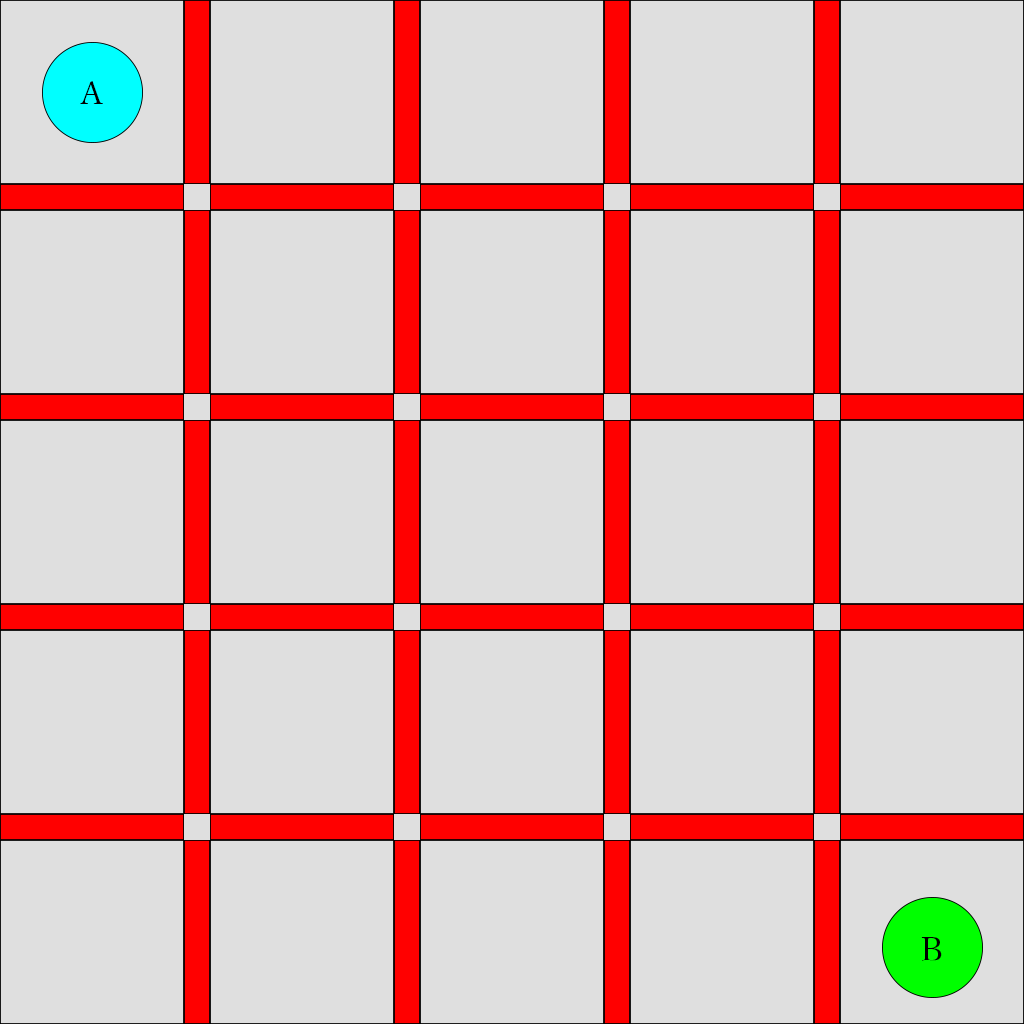
\includegraphics[width=0.4\textwidth]{Gameboard.png}
    \caption{Gameboard}
\end{figure}

\subsection{Setup}

At first, players A and B are randomly positioned on the chessboard symmetrically. 
%
The two players will take turns to move in the chessboard and put barriers.
%
In each turn, one player will move \textbf{at most} $K$ steps and \textbf{must} put a barrier in one of the 4 directions around itself at the end of moving. Here, $K$ is computed as $\lfloor\frac{M+1}{2}\rfloor$, which defines the maximum number of allowable steps. 
%
Each step can only be made horizontally or vertically.
%
One player cannot go into the other's position, go through the barriers, or put barriers in places that already have barriers (including the game borders). To increase the randomness of the game, $K*2$ barriers will be initially put on the chessboard in a symmetrically.

\subsection{Objective}

The game ends when two players are separated into two closed zones by barriers and borders.
The final score of each player is \textit{the number of blocks in its zone in the endgame}.
%
The player with the higher score will win the game, and will be awarded 1 point.
If there is a tie, both players will be awarded 0.5 points. An example gameplay is shown in Figure \ref{example_game}.

\subsection{Playing the game}

For each step, the move consists of providing an (x,y) co-ordinate of the board where the player wants to go, and a direction (up/right/down/left) the player wants to put a wall. The number of steps taken to go to position (x,y) will be automatically computed by the game engine using a breadth-first-search algorithm, and if the steps are more than $K$ then errors will be shown.

\subsection{Evaluation}

In the first round of the evaluation, we will hold a competition where every submitted program will be playing one match against a random subset of all submissions. Due to the deterministic nature of the game board, each match will consist of $N$ games, giving both programs equal opportunity to play first (typically $N>1000$). For the second round, the 10 percent highest scoring agents from the first game will play against each other in the playoff round where each agent is paired against all other agents to find the highest scoring agents. The evaluation phase will require a lot of matches so please be mindful of your program’s runtime. We will perform a screening process by pairing your agent with a random agent to ensure the runtimes matches the expectations (check the Tournament Constraints in Section \ref{sec:tournament_constraints}).


\begin{figure}[ht!]%
\centering
\subfloat[Step 0]{
    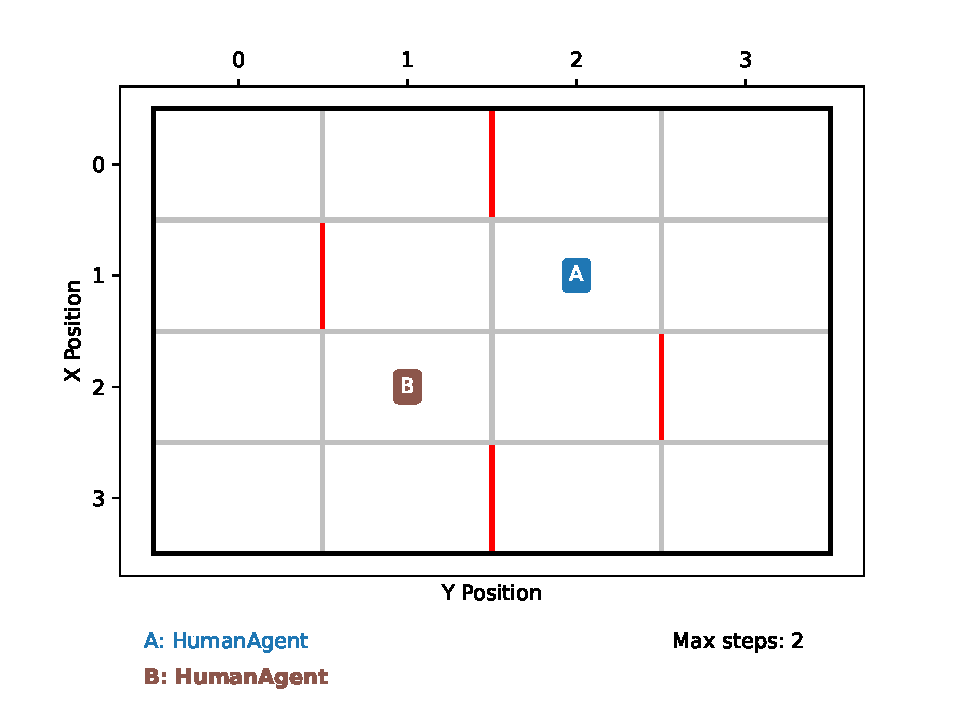
\includegraphics[width=0.48\linewidth]{figs/human_agent_human_agent_0.pdf}\hfill
}
\subfloat[Step 1]{
    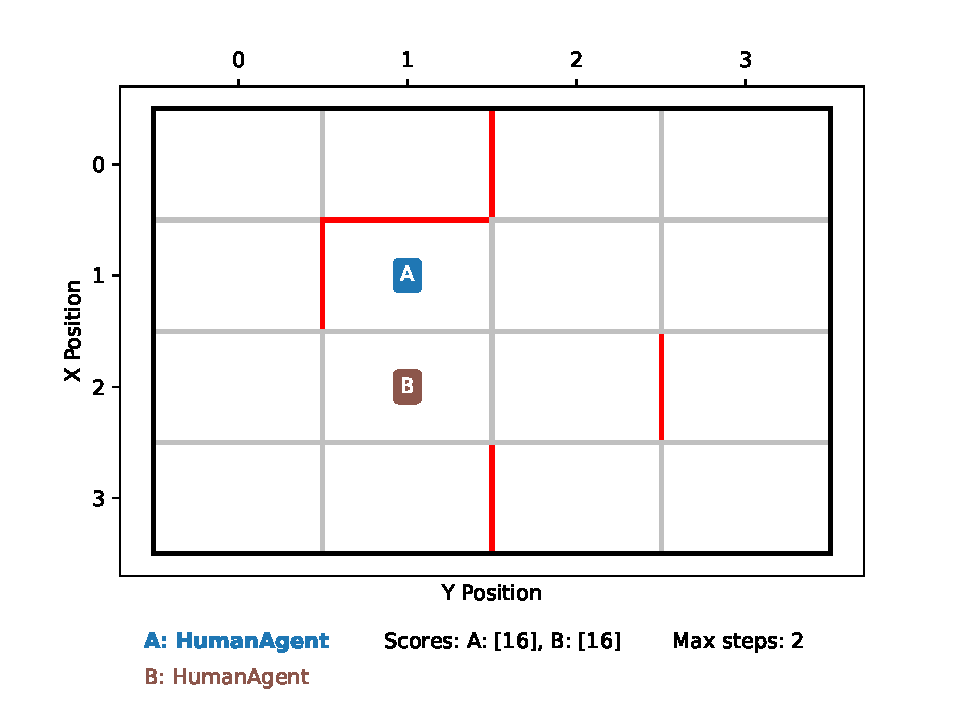
\includegraphics[width=0.48\linewidth]{figs/human_agent_human_agent_1.pdf}\hfill
} \\
\subfloat[Step 2]{
    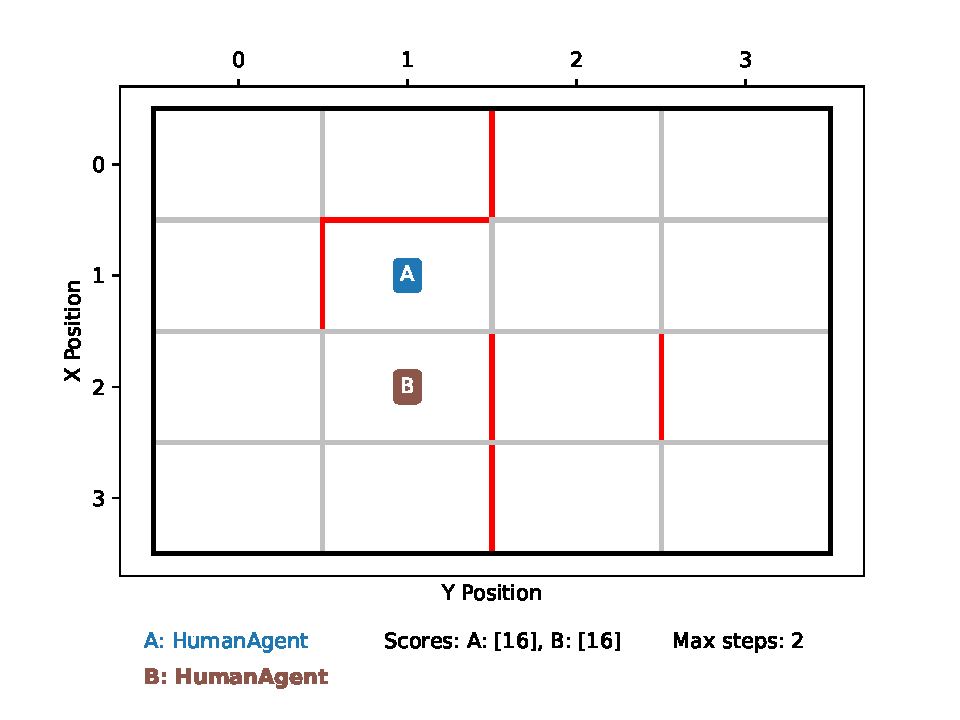
\includegraphics[width=0.48\linewidth]{figs/human_agent_human_agent_2.pdf}
}\hfill
\subfloat[Step 3]{
    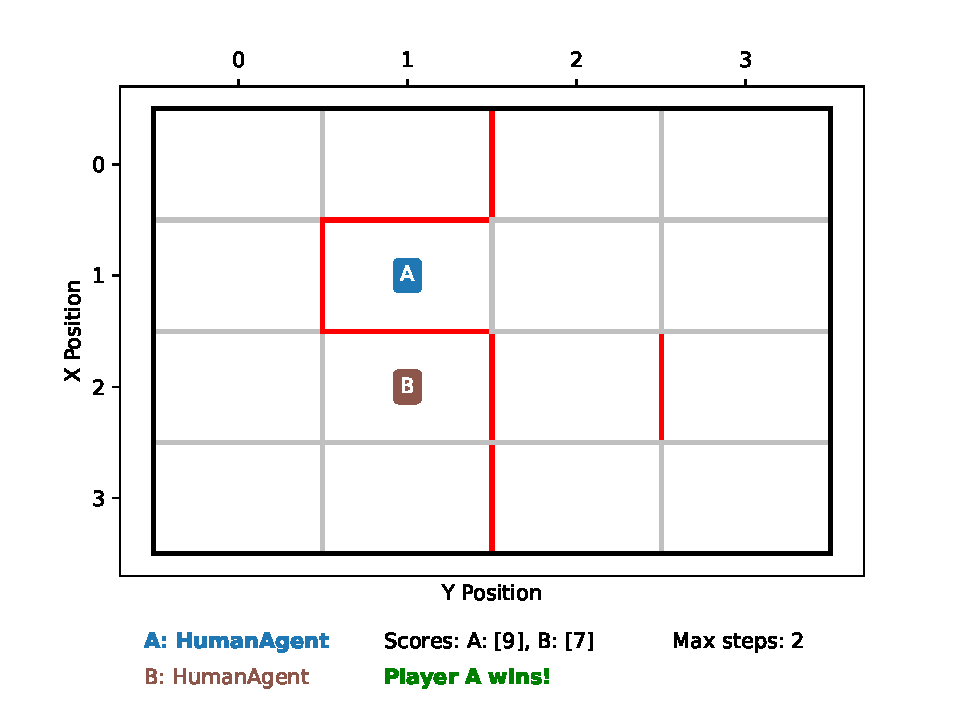
\includegraphics[width=0.48\linewidth]{figs/human_agent_human_agent_3.pdf}
}
\caption{A sample game between two agents (A and B) on a 4x4 chessboard, thus having max allowable steps $K=2$. The board is initialized (Step 0) with random (symmetrical) wall placements. A then moves to position $(1,1)$ and places a wall on the \textit{top} (Step 1). B remains in the same position $(2,1)$ and places a wall on the \textit{right} (Step 2). A then wins the game by staying in the same position $(1,1)$ and placing a wall on \textit{down}, thus having control of 9 blocks in the board (Step 3). }
\label{example_game}
\end{figure}

\section{Assignment Details}

In this final project, your task is to develop an \textit{agent} to play the \textit{Colosseum Survival} game. We have developed a minimalistic game engine in Python, which you will extend to add your own \textit{agents}. 

\subsection{Pre-requirements}

This project you will need to implement agent that playes Colosseum Survival using Python. Specifically, we strongly recommend to brush up Python 3 fundamentals before writing your code. We would also require you to know \texttt{git} fundamentals to work with the version control system, and have an account in \href{https://github.com}{Github}.

\subsection{Working with Github Classrooms}

For the purposes of this project, we will be using Github Classrooms. Github Classrooms allow us to easily share the template repository and create private repositories for students. To start working in your assignment:

\begin{itemize}
    \item Accept this invitation (\textbf{\href{https://classroom.github.com/a/dRpR9fvL}{https://classroom.github.com/a/dRpR9fvL}}) to be added to our COMP 424 Github Classroom. Please register your team by \textbf{March 11th, Friday}.
    \item Choose or create your team. Teams can be formed only with \textbf{two} members.
    \item Once you accept the assignment, your code repository will be setup using the starter code. 
    \item In your repository, a Pull Request (PR) would be automatically created, which would serve as a way to communicate with the TAs about specific, private concerns regarding your code or to get feedback. Alternatively, you can contact the TAs involved in this project directly.
    \item Clone your assigned repository to start working on the assignment \footnote{Check the detailed description of the files in the repository in Section \ref{sec:repository}}.
    \item Navigate to the cloned directory and install the dependencies : \texttt{pip install -r requirements.txt}
    \item To test that everything runs on your machine as required, run the following command in the cloned directory: \texttt{pytest}
\end{itemize}

\subsection{Implementing your own agent}

You need to write your own \textit{agent} and submit it for the class project. Detailed instructions of various parts of the game is available in the \textbf{README.md} file. Follow the steps to implement and test your own agent:

\begin{itemize}
    \item Modify the 
    \texttt{student\_agent.py} file in \texttt{agents/} directory, which extends the \texttt{agents.Agent} (in \texttt{agents/agent.py}) class.
    \item Implement the step function with your game logic
    \item Register your agent using the decorator \texttt{register\_agent}. The \texttt{StudentAgent} class is already decorated with the name \textit{``student\_agent"}, feel free to change it or keep it the same.
    \item Import your agent in the \texttt{\_\_init\_\_.py} file in \texttt{agents/} directory. This step is already done for \texttt{StudentAgent}.
    \item Run and test your agent using \texttt{simulator.py} script.
\end{itemize}

\noindent \textbf{Important}: You should not modify any other files apart from \texttt{student\_agent.py} and any helper file you need should also be created within \texttt{agents/} directory. In the event of any update to the game code, the TAs will announce the necessary steps in Ed to pull the starter code.

\subsection{Play with your agent}

You can use the \texttt{simulator.py} script to run an interactive session with your agent! A Human agent (yourself) is defined in \texttt{agents/} directory, along with a random walk agent. You can first \textit{visualize} the game happening between the two agents as follows:

\begin{verbatim}
python simulator.py \
  --player_1 human_agent \
  --player_2 random_agent \
  --display
\end{verbatim}

You can play with your agent likewise by using the name you \textit{registered} your agent with (e.g. \textit{``student\_agent"}). To quickly play the game without displaying the UI, remove the \texttt{--display} flag.

\subsection{Testing and Autoplay}

Since the game setup is non-deterministic, your submitted agent will be evaluated on multiple runs by playing them against the \texttt{random\_agent} or other student submissions. This is achieved by the autoplay mode, enabled by \texttt{--autoplay} flag in \texttt{simulator.py}. Thus, it is crucial that you test your agent against the \texttt{random\_agent} before submitting your work. You can play with the flag \texttt{--autoplay\_runs} to set the number of simulations. In autoplay mode, the starting agent is swapped every other run, so as to remove the disadvantage of starting first in the game.

During autoplay, if your agent does not adhere to the boundary conditions of the board, or attempts to make an invalid move (more than $K$ steps), the game engine will automatically run a \textit{random walk} on behalf of your agent. This may adversely affect your agents performance during evaluation. You should test your agent thoroughly for these edge cases.

\subsection{Submission}

First, fill your and your team members details in \texttt{authors.yaml} file in the repository.
You should periodically \texttt{commit} your code and push it to the repository assigned to you.
Your code will be automatically deemed submitted post the deadline date. You can continue to make changes in the Github Classroom repository before the deadline. Any changes post the deadline will not be used for the final evaluation.

\section{Report}

You are required to write a report with a detailed explanation of your approach and reasoning. The report must be a typed PDF file, and should be free of spelling and grammar errors. The suggested length is between 4 and 8 pages, but the most important constraint is that the report be clear and concise. You should use the source of this document \footnote{You can find the source of this document in Overleaf here: \href{https://www.overleaf.com/read/gcpfjdpqpytp}{https://www.overleaf.com/read/gcpfjdpqpytp}. You would need to create an Overleaf account. Copy this project and create a new project to write your report. Replace the \texttt{author} information with your own group information.} as a template to write your report in \LaTeX.  The report must include the following required components:

\begin{itemize}
    \item An explanation of how your program works, and a motivation for your approach.
    \item A brief description of the theoretical basis of the approach (about a half-page in most cases); references to the text of other documents, such as the textbook, are appropriate but not absolutely necessary. If you use algorithms from other sources, briefly describe the algorithm and be sure to cite your source.
    \item A summary of the advantages and disadvantages of your approach, expected failure modes, or weaknesses of your program.
    \item If you tried other approaches during the course of the project, summarize them briefly and discuss how they compared to your final approach.
    \item A brief description (max. half page) of how you would go about improving your player (e.g. by introducing other AI techniques, changing internal representation etc.)
    
\end{itemize}

\subsection{Submission}

To submit your report, you should also add the report PDF directly in the repository in the \texttt{report} folder, rename it to \texttt{report.pdf}, and commit and push your report alongside with your code.

\section{Grading Scheme}

50\% of the project grade will be allotted for performance in the tournament, and the other 50\% will be based on your report.

\subsection{Tournament Grading Scheme}

The top scoring agent will receive full marks for the tournament. The remaining agents will receive marks according to a linear interpolation scheme based on the number of wins/losses they achieve. To get a passing grade on the tournament portion, your agent must beat the random player.

\subsubsection{Tournament Constraints}
\label{sec:tournament_constraints}

During the tournament, we will use the following additional rules:

\begin{itemize}
    \item \textbf{Execution Environment}. We will run the tournament on Linux environment (CentOS 7), Python 3.9 and install libraries as defined in \texttt{requirements.txt}. However, you are not allowed to use external libraries. This means built-in libraries for computation are allowed but libraries made specifically for machine learning or AI are not. If you think you would require some external libraries not specified in \texttt{requirements.txt} and which is not a AI/ML specific library, please post a question in Ed to get an approval from the TAs.

    \item \textbf{Turn Timeouts}. During each game, your agent will be given no more than 30 seconds to choose its First move, and no more than 2 seconds to choose each subsequent move. The initial 30 second period should be used to perform any setup required by your agent (e.g. any pre-processing step). If your player does not choose a move within the allotted time, a random move will be chosen instead. If your agent exceeds the time limit drastically (for example, if it gets stuck in an infinite loop) then you will suffer an automatic game loss.
    
    \item \textbf{Illegal moves}. In the game, if your agent attempts to move to positions which are illegal, i.e. which requires more number of steps than $K$, then we will run a random walk over the game board. If your code fails during execution, then the game will also continue with a random move.
    
    \item \textbf{Multi-threading}. Your agent will be allowed to use multiple threads. However, your agent will be confined to a single processor, so the threads will not run in parallel. Also, you are required to halt your threads at the end of your turn (so you cannot be computing while your opponent is choosing their move).
    
    \item \textbf{File IO}. Your player will not be allowed to read and write files : all file IO is prohibited. In particular, you are not allowed to write files, so your agent will not be able to do any learning from game to game.
    
    \item \textbf{Memory Usage}. Your agent will run in its own process and will not be allowed to exceed 500 mb of RAM.  Exceeding the RAM limits will result in a game loss. 
    
\end{itemize}

You are free to implement any method of choosing moves as long as your program runs within these constraints and is well documented in both the write-up and the code. Documentation is an important part of software development, so we expect well-commented code. All implementation must be your own. 

\subsection{Report Grading Scheme}

The marks for the write-up will be awarded as follows:

\begin{itemize}
    \item Technical Approach: 20/50
    \item Motivation for Technical Approach: 10/50
    \item Pros/cons of Chosen Approach: 5/50
    \item Future Improvements: 5/50
    \item Language and Writing: 5/50
    \item Organization: 5/50
\end{itemize}



% \subsection{Tournament Evaluation}

% Your submitted code will be played against your peer's submission in a \textit{tournament} mode. 
% In tournament mode, we will run your agent against another student's agent in \texttt{autoplay} mode with $N$ evaluations (where $N$ is a hidden number).
% More details about the schedule of the tournament will be announced closer to the submission deadline date.

\section{Academic Integrity}

This is a group project. The exchange of ideas regarding the game is encouraged, but sharing of code and reports is forbidden and will be treated as cheating. We will be using document and code comparison tools to verify that the submitted materials are the work of the authors only. Please see the syllabus and \href{www.mcgill.ca/integrity}{www.mcgill.ca/integrity} for more information.

\section{Contact}

Feel free to contact the TA's if you have any specific concern that needs to be addressed.

\begin{itemize}
    \item Koustuv Sinha, koustuv.sinha@mail.mcgill.ca
    \item Shuhao Zheng, shuhao.zheng@mail.mcgill.ca 
\end{itemize}

\section{Detailed description of the repository}
\label{sec:repository}

The starter code can be viewable here: \href{https://github.com/Ctree35/Project-COMP424-2022-Winter}{https://github.com/Ctree35/ Project-COMP424-2022-Winter}. The following describes the usage of each component of this code:

\begin{verbatim}
 |-store.py             # Storing agents for decorator
 |-world.py             # Main Game engine code
 |-requirements.txt     # Specify external libraries to be installed used pip
 |-test                 # Unit test files
 | |-conftest.py
 | |-test_agent.py      # Test case for AI agents
 | |-test_world.py      # Test case for game engine
 |-ui.py                # UI Engine files
 |-authors.yaml         # Students should fill out author information
 |-constants.py         # Handy constants for the game
 |-agents               # Directory containing all agents
 | |-random_agent.py    # Agent that takes random walk
 | |-__init__.py        # All agents should be imported here
 | |-human_agent.py     # Human agent using which you can play interactively
 | |-agent.py           # Base agent class
 | |-student_agent.py   # Implement your AI here
 |-README.md
 |-utils.py             # Some utilities for the game
 |-simulator.py         # Main entry point for running the game
 |-report               # Upload your report in this directory
 | |-README.md
\end{verbatim}





% \vskip 0.2in
% \bibliography{sample}

\end{document}